\section{Definitions of Useful Quantities}

In the energy landscapes view, a ``species" is a useful yet artificial concept discretising the configuration space.
A proper definition of species is essential for accurately describing any process on the landscape.
For example, in TPS \cite{Dellago1998b} studies of a cluster of Lennard-Jones discs, small spheres in RMSD space surrounding the minima were used.
A convenient definition used in DPS assigns regions in configuration space to the basins of attraction of particular local minima.\cite{Wales2003}
Dividing surfaces then roughly agree with the maxima on the transition pathways.
However, assignment of a structure to the corresponding minimum can be computationally expensive and the number of boxes also corresponds to the number of minima, which grows roughly exponentially with the number of particles.
Another method of partitioning the space is Voronoi tesselation in which phase points are assigned to one of the boxes using a selected measure.
As well as partitioning along a collective coordinate, the Voronoi method seems to be the most convenient for master equation modelling since it describes all states of the system, so the sum of the populations is conserved in any process, and in principle it allows an arbitrary number of boxes.
The dividing surface is unambiguously defined and the transmission coefficient is unity (see figure \ref{fig:recross}).

\begin{figure}[h]
\centering
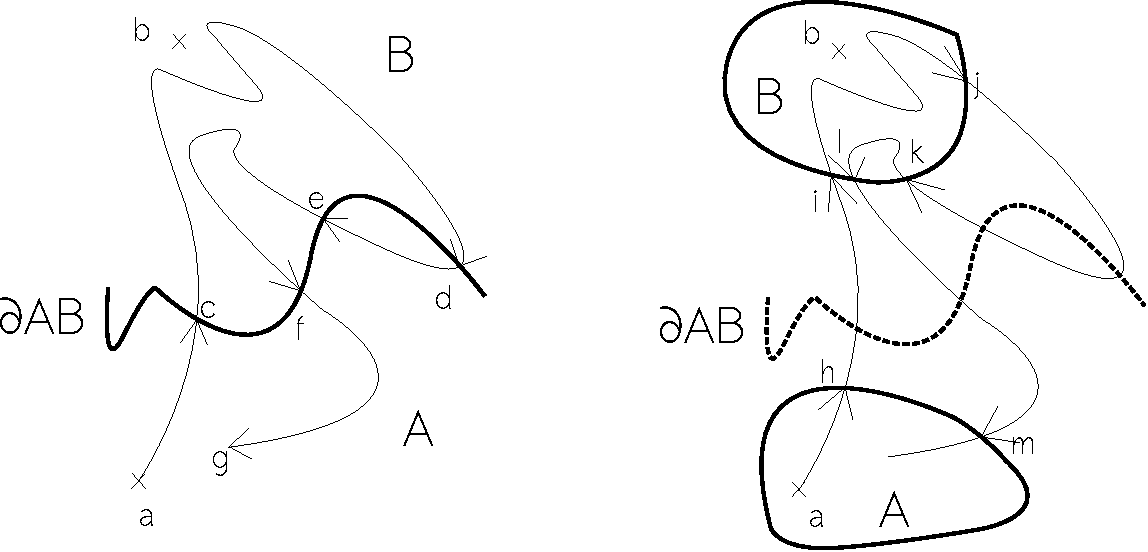
\includegraphics[width=14cm]{Images/recrossing.pdf}
\caption[Comparison of species definitions.]{Comparison of the species definition used in BXD (left) and TPS (right). Thick full line defines the species, dashed line represents the dividing surface and the thin line represents a trajectory obtained from a simulation. Points a and b are minima on the PES. Points c to m divide the trajectories into subtrajectories. {\bf Left:} All trajectories crossing the dividing surface (a-c, c-d, d-e and e-f) except for f-g are reactive since at their ends the particle becomes a different species. The transmission coefficient is unity for a simulation that ends at the dividing surface (a-f). {\bf Right:} h-i and l-m are reactive trajectories and j-k is a non-reactive trajectory. The total population of states at times the particle is outside the boxes (h-i, j-k, l-m) is lower than at times the particle is inside either of the boxes (a-h, i-j, k-l).}
\label{fig:recross}
\end{figure}


In the master equation, a transition from any state A to a different state B is assumed to be a Poisson process.
Any memory of previous processes is completely lost.
Therefore, a standard distribution of states inside a particular box must be defined.
Any property of species A can be calculated as the mean property of all states in box A using this distribution.
A natural, and perhaps the most convenient choice, is the equilibrium distribution.
A transition from box A to box B can then be described by an ensemble of trajectories with starting points evenly (in the microcanonical ensemble) distributed in A and endpoints evenly distributed in B.

Now let us define some useful quantities used in the following discussions in microcanonical ensemble.
The box phase volume, \(\Gamma_{\rm A}\), is
\begin{equation}
\label{eq:gamma}
\Gamma_{\rm A }
= \int_{{\bf q} \in A} \!\!\!\!\! 1 ~ {\rm d}{\bf p} {\rm d}{\bf q} 
= \int \! H({\bf q}, A) ~ {\rm d}{\bf p} {\rm d}{\bf q} \rm ~,
\end{equation}
where $H({\bf q}, A)$ is one if ${\bf q}$ lies in A and zero otherwise.
The equilibrium probability of being in box A, $P_{\rm A}$, is given simply by the ratio of its volume to the total volume of all the boxes

\begin{equation}
\label{eq:prob}
P_{\rm A }
= \frac{\Gamma_{\rm A }}{\sum_{\rm i} \Gamma_{\rm i}} ~.
\end{equation}
The non-equilibrium population of states in box A at time $t$ is given by

\begin{equation}
\mathscr{P}_{\rm A}(t) = \int_{{\bf q} \in A} \!\!\!\!\! \rho ({\bf p},{\bf q}, t ) ~ {\rm d}{\bf p} {\rm d}{\bf q} 
= \int \! \rho ({\bf p},{\bf q}, t ) ~ H({\bf q} , A) ~ {\rm d}{\bf p} {\rm d}{\bf q} ~ ,
\end{equation}
where $\rho_{eq}({\bf p},{\bf q},t)$ is the probability of state $({\bf p},{\bf q})$ at time $t$.
The probability of being in box A at time $t$, which is the central quantity for master equation modelling, is 

\begin{equation}
\label{eq:probt}
P_{\rm A } (t)
= \frac{\mathscr{P}_{\rm A }(t)}{\sum_{\rm i} \mathscr{P}_{\rm i} (t)} ~.
\end{equation}

For each phase point $({\bf p},{\bf q} )$ in A we can define the first passage time (FPT) $t^{fp}_{\rm A \rightarrow \partial AB}$ as the time it takes for the trajectory starting from $({\bf p},{\bf q} )$ to reach any phase point in the boundary $\rm \partial AB$.
The flux through the dividing surface between A and B, $\partial \rm AB$, at time $t$ can be defined by the population of states as follows:
let us consider a system in which configuration space is divided into two boxes A and B only.
Let all the trajectories leaving B through the dividing surface at time $t_0$ be reflected back to box B.
The rate of change of population of states in B is given by the flux through the boundary surface $\rm \partial AB$

\begin{equation}
\label{eq:def-flux}
\mathscr{F}_{\rm A \rightarrow \partial AB } (t_0)
= \frac{\partial}{\partial t} \mathscr{P}_{\rm B } (t) |_{t=t_0} ~.
\end{equation}
The normalised flux can be defined in a similar way as:

\begin{equation}
\label{eq:def-flux-norm}
F_{\rm A \rightarrow \partial AB } (t_0)
= \frac{\partial}{\partial t} P_{\rm B } (t) |_{t=t_0} 
= \frac{\mathscr{F}_{\rm A \rightarrow \partial AB } (t_0)}{\mathscr{P}_{\rm A} (t_0)} ~.
\end{equation}
This flux between the boxes in equilibrium is used in TST for the definition of the rate constants.
The rate coefficient $\varkappa_{\rm A \rightarrow \partial AB}$ can be defined at time $t_0$ as 

\begin{equation}
\label{eq:ratecoeff}
{\varkappa}_{\rm A \rightarrow \partial AB } (t_0)
= \frac{\mathscr{F}_{\rm A \rightarrow \partial AB } (t_0)}{\mathscr{P}_{\rm A} (t_0)}
= \frac{F_{\rm A \rightarrow \partial AB } (t_0)}{P_{\rm A} (t_0)} ~.
\end{equation}
Master equation modelling assumes this quantity to be independent of time.
If we assume that the states in B are in equilibrium with the others lying on the same trajectory at all times, the flux $F_{\rm A \rightarrow \partial AB } (t_0)$ is formally equivalent to the reaction rate $v_{\rm A \rightarrow B}$ [see equation (\ref{eq:v})] and ${\varkappa}_{\rm A \rightarrow \partial AB } (t_0)$ is the rate constant.

